\documentclass{article}

\usepackage{geometry}
\usepackage{graphicx}

\title{Exercise 1, TFY4235 Computational physics}
\author{Martin K. Johnsrud}
\vspace{-8ex}
\date{}


\begin{document}
    \maketitle
    \section*{Introduction}
        The goal of this exercise is to simulate particles as flat, hard disks in a square, 2D container. This is done with a event-driven simulation, as described in the exercise~\cite{exercise}. This is implemented in Python, using the built-in library heapq. The simulation is used to first tested with scenarios we know the outcome of, then used to demonstrate the Maxwell-Boltzmann distribution and to investigate the effect of a large, heavy disk hitting a large number of small, inert particles.
    
    \section*{Implementation}
        The main engine of the code is the function \verb|run_loop()| in \verb|utillities.py|. It follows the algorithm, as laid out in~\cite{exercise}, using the objects:
        \begin{itemize}
            \item \verb|particles|, a numpy array with the position and velocity of all the particles.
            \item \verb|collisions|, a priority queue containing the time of the collision, the index of the particle(s) involved, and the type of collision it is.
            \item \verb|last_collided|, a list of when each particle was involved in a collision.
        \end{itemize}
        To be expanded \dots

    \section*{Tests}
    Several functions were developed to test the accuracy of the simulation. First, one particle, starting at in the middle of the box, all the way to the left, and with a velocity with at $45^\circ$ to the $x$-axis should move in a titled rectangle. With $\xi=1$ it should also conserve energy.

    \begin{figure}
        \centering
        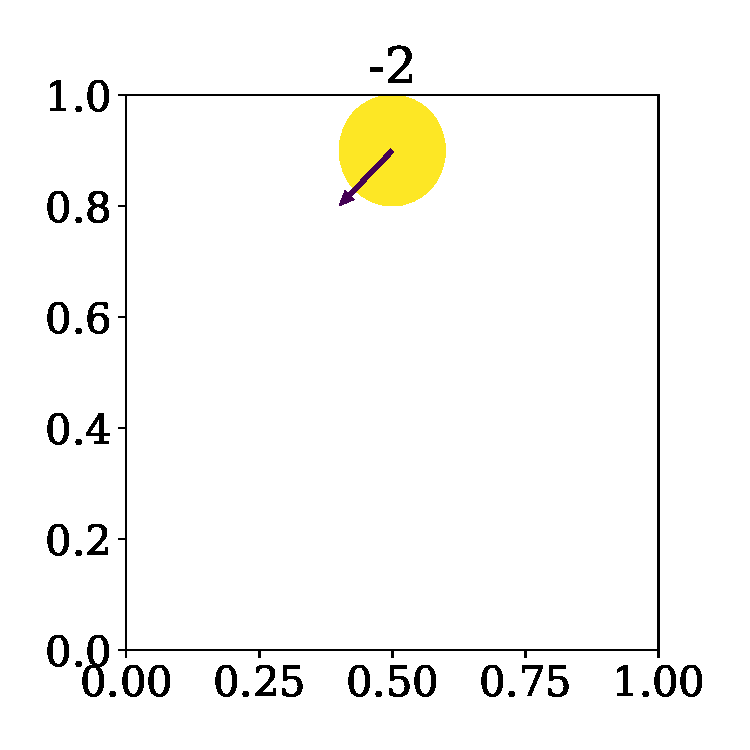
\includegraphics[width=0.49\textwidth]{../plots/test_case_one_particle/particle-2.pdf}
        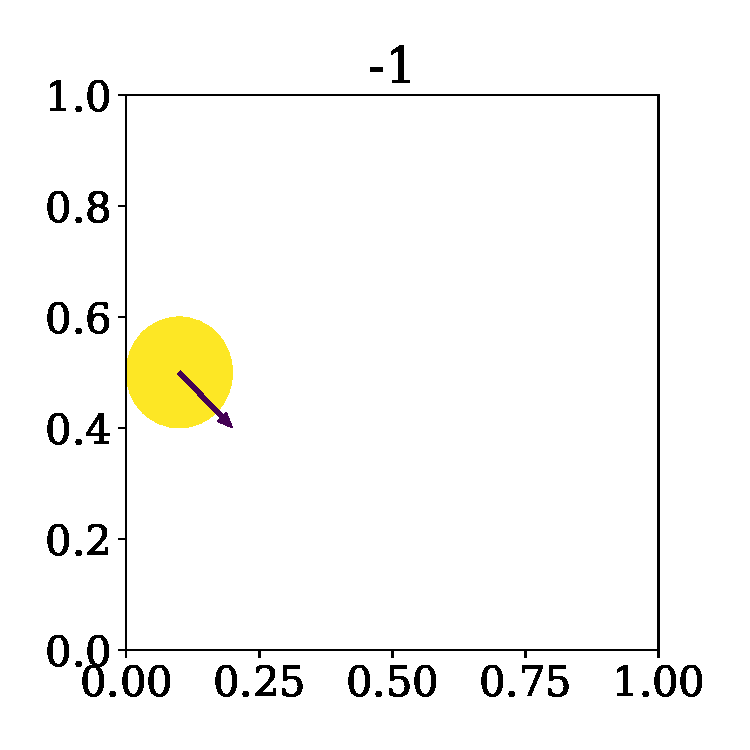
\includegraphics[width=0.49\textwidth]{../plots/test_case_one_particle/particle-1.pdf}
        \caption{One ball being simulated. after $10 000$ steps, it still follows a regular pattern.}
    \end{figure}


    \bibliography{report}
    \bibliographystyle{plain}   
\end{document}